% ============================================================ Capítulo: versión 2.0 — simulador 3D
\chapter{Versión 2.0: simulador 3D de ensamblajes}\label{cap:simulador}

\section{Objetivo y alcance}
La versión~2.0 agrega un simulador 3D web de ensamblajes de autopartes con el \textbf{freno de disco} como caso
principal. El simulador permite explorar la jerarquía de piezas, sus articulaciones, la vista de despiece y
reensamblaje y un cálculo simplificado del frenado, e integra la base de conocimiento para responder preguntas por
pieza. Streamlit continúa como interfaz empresarial principal y enlaza o incrusta el visor.

\begin{nota}[Carácter demostrativo]
La geometría es procedural y simplificada, y las dimensiones y coeficientes están marcados como
\texttt{demostrativo}. No constituye un diseño industrial certificado, la animación no valida propiedades mecánicas
y el sistema no genera procedimientos de reparación ni de seguridad. Los modelos de Claude no sustituyen el motor
geométrico (trimesh + manifold3d), el cálculo físico ni un software CAD.
\end{nota}

\section{Arquitectura}
\begin{figure}[H]\centering
\begin{tikzpicture}[every node/.style={font=\sffamily\scriptsize}]
  % paquete simulador
  \node[caja=2.6cm] (mod) at (0,0) {\texttt{modelos.py}\\Pieza, Articulación};
  \node[caja=2.6cm] (cat) at (3.05,0) {\texttt{catalogo\_freno.py}\\15 piezas, 15 artic.};
  \node[caja=2.6cm] (cin) at (6.1,0) {\texttt{cinematica.py}\\Rodrigues, despiece, Kahn};
  \node[caja=2.6cm] (fis) at (9.15,0) {\texttt{fisica\_freno.py}\\$T = 2\mu pAr$};
  \node[caja=2.6cm] (gen) at (3.05,-1.5) {\texttt{generacion.py}\\trimesh + manifold3d};
  \begin{scope}[on background layer]
    \node[grupo=fnagris, fit=(mod)(cat)(cin)(fis)(gen), label={[font=\sffamily\scriptsize\bfseries]above:paquete \texttt{simulador} (sin dependencias de capas superiores)}] {};
  \end{scope}
  % servicios y datos
  \node[almacen, minimum width=2.4cm] (glb) at (3.05,-3.6) {freno\_disco.glb\\+ manifiesto};
  \node[clave=2.6cm] (svc) at (7.25,-3.6) {ServicioSimulador\\biblioteca de máquinas};
  \node[almacen, minimum width=2.3cm, fill=oro!20] (kb) at (11.6,-3.6) {Base Gold\\(scraping)};
  \node[caja=2.6cm] (api) at (7.25,-5.4) {FastAPI\\\texttt{/api/v1/simulador}};
  \node[almacen, minimum width=2.3cm] (db) at (11.6,-5.4) {SQLite /\\PostgreSQL};
  % interfaces
  \node[caja=2.3cm] (st) at (0,-7.3) {Streamlit\\(iframe y enlaces)};
  \node[caja=2.8cm, fill=fnaazul!8, draw=fnaazul] (web) at (4.2,-7.3) {Visor React Three Fiber\\\texttt{/app}};
  \node[caja=2.3cm] (mcp) at (11.6,-7.3) {MCP\\\texttt{consultar\_pieza}};
  % flechas
  \draw[flecha] (cat) -- (gen);
  \draw[flecha] (gen) -- (glb);
  \draw[flecha] (cin.south) -- (svc.north west);
  \draw[flecha] (fis.south) -- (svc.north east);
  \draw[flecha] (kb) -- (svc);
  \draw[flecha] (svc) -- (api);
  \draw[flecha] (api) -- (db);
  \draw[flecha] (api.south west) -- (web.north east);
  \draw[flecha] (glb.south) -- node[etq, left, pos=0.45]{GLB estático} (web.north west);
  \draw[flecha] (st) -- (web);
  \draw[flechad] (svc.south east) -- (mcp.north west);
\end{tikzpicture}
\caption{Arquitectura del simulador 3D y su integración con el sistema}\label{fig:sim-arquitectura}
\end{figure}

El paquete \texttt{simulador} depende solo de la biblioteca estándar, Pydantic, numpy y trimesh; la verificación de
capas (\texttt{scripts/verificar\_capas.py}) lo ubica por debajo de \texttt{services}. El visor se compila con Vite a
\ruta{web/dist} y FastAPI lo sirve en \texttt{/app}, en el mismo origen que la API.

\section{Modelo de componentes}
\begin{figure}[H]\centering
\begin{tikzpicture}[clase/.style={rectangle split, rectangle split parts=2, draw=fnagris, fill=white,
    font=\sffamily\scriptsize, align=left, text width=#1, rectangle split part fill={fnaazul!10,white}},
    clase/.default=4.4cm]
  \node[clase] (ens) at (0,0) {\textbf{Ensamblaje}\nodepart{second}id, nombre, versión, parámetros, procedencia\\piezas[ ], articulaciones[ ], subconjuntos[ ]\\advertencia};
  \node[clase=3.6cm] (sub) at (7.2,0.3) {\textbf{Subconjunto}\nodepart{second}id, nombre, piezas[ ]};
  \node[clase=5.4cm] (pie) at (0,-3.7) {\textbf{Pieza}\nodepart{second}id, nombre, tipo, función, material\\dimensiones\_m, geometría, transformación\\ancla, subconjunto, relacionadas[ ]\\dirección\_despiece, distancia\_despiece\_m\\retirar\_antes[ ], visible, metadatos\\referencia\_documental};
  \node[clase=5.2cm] (art) at (7.2,-3.4) {\textbf{Articulación}\nodepart{second}id, tipo: fija | rotacional | prismática |\\esférica | compuesta\\padre, hijo, eje unitario, origen\\límites o continua, unidad\\maestra y relación (compuesta)};
  \node[clase=3.6cm] (geo) at (-1.2,-7.3) {\textbf{Geometría}\nodepart{second}primitiva, parámetros $>$ 0\\nodo\_glb, color};
  \node[clase=3.6cm] (tra) at (3.4,-7.3) {\textbf{Transformación}\nodepart{second}posición (m)\\rotación\_grados (Euler XYZ)};
  \draw[thick] (ens.east) -- node[etq,above,pos=0.15]{1} node[etq,above,pos=0.85]{1..*} (sub.west |- ens.east);
  \draw[thick] (ens.south) -- node[etq,right,pos=0.2]{1} node[etq,right,pos=0.8]{1..*} (pie.north);
  \draw[thick] (ens.east) ++(0,-0.45) -| node[etq,right,pos=0.85]{1..*} (art.north);
  \draw[thick] (pie.south) ++(-1.2,0) -- node[etq,right]{1} (geo.north);
  \draw[thick] (pie.south) ++(1.6,0) -- node[etq,right]{1} (tra.north);
  \draw[thick,dashed] (art.west) -- node[etq,above]{padre / hijo} (pie.east |- art.west);
\end{tikzpicture}
\caption{Modelo de componentes (Pydantic) del simulador}\label{fig:sim-modelo}
\end{figure}

\begin{table}[H]\centering\small
\caption{Validaciones del modelo de componentes}\label{tab:sim-validaciones}
\begin{tabularx}{\linewidth}{@{}P{4.2cm} X@{}}\toprule
Regla & Efecto\\\midrule
Identificador \verb|^[a-z][a-z0-9_]*$| y único & Nodos GLB, rutas de la API y árbol del visor coherentes.\\
Parámetros geométricos positivos & Mallas cerradas con volumen positivo.\\
Eje unitario y límites (o \texttt{continua}) & Rechazo de articulaciones mal definidas.\\
Compuesta con \texttt{maestra} y \texttt{relación} & Movimiento derivado y trazable.\\
\texttt{retirar\_antes} sin ciclos ni referencias rotas & Secuencia de desmontaje siempre calculable.\\
\texttt{distancia\_despiece\_m} en (0, 1] & Despiece acotado y reversible.\\\bottomrule
\end{tabularx}
\end{table}

\section{Jerarquía del freno de disco}
\begin{figure}[H]\centering
\begin{tikzpicture}[grow'=right, level distance=3.4cm,
    level 1/.style={sibling distance=2.4cm},
    level 2/.style={sibling distance=0.48cm},
    every node/.style={font=\sffamily\scriptsize, anchor=west},
    edge from parent/.style={draw=fnagris, thin},
    edge from parent path={(\tikzparentnode.east) -- ++(0.2,0) |- (\tikzchildnode.west)}]
  \node[clave=2.3cm, anchor=center] {freno\_disco\\(ensamblaje)}
    child {node[caja=2.0cm, anchor=west] {rotación}
      child {node {cubo}}
      child {node {disco}}
      child {node {esparrago\_1 \dots\ esparrago\_4}}
    }
    child {node[caja=2.0cm, anchor=west] {pinza}
      child {node {soporte\_pinza}}
      child {node {cuerpo\_pinza}}
      child {node {piston}}
      child {node {pastilla\_interna}}
      child {node {pastilla\_externa}}
      child {node {pasador\_guia\_1, pasador\_guia\_2}}
    }
    child {node[caja=2.0cm, anchor=west] {fijación}
      child {node {tornillo\_soporte\_1, tornillo\_soporte\_2}}
    };
\end{tikzpicture}
\caption{Jerarquía del ensamblaje: subconjuntos y piezas}\label{fig:sim-jerarquia}
\end{figure}

\section{Articulaciones}
\begin{figure}[H]\centering
\begin{tikzpicture}[every node/.style={font=\sffamily\scriptsize}, lbl/.style={etq, align=center}]
  \node[externo=1.9cm] (mundo) at (0,0) {mundo\\(mangueta)};
  \node[caja=1.9cm] (cubo) at (5.6,0) {cubo};
  \node[caja=1.9cm] (disco) at (11.2,0) {disco};
  \node[caja=1.9cm] (sop) at (0,-2.4) {soporte\_pinza};
  \node[caja=1.9cm] (cuerpo) at (5.6,-2.4) {cuerpo\_pinza};
  \node[caja=1.9cm] (piston) at (11.2,-2.4) {pistón};
  \node[caja=2.1cm] (pe) at (5.6,-4.6) {pastilla\_externa};
  \node[caja=2.1cm] (pi) at (11.2,-4.6) {pastilla\_interna};
  \draw[flecha] (mundo) -- node[lbl,above]{j\_rueda\\rotacional, continua, eje $z$} (cubo);
  \draw[flecha] (cubo) -- node[lbl,above]{j\_disco\_cubo\\fija} (disco);
  \draw[flecha] (mundo) -- node[lbl,right]{j\_soporte · fija} (sop);
  \draw[flecha] (sop) -- node[lbl,above]{j\_pinza\_flotante\\prismática $-z$, 0--3\,mm} (cuerpo);
  \draw[flecha] (cuerpo) -- node[lbl,above]{j\_piston\\prismática $+z$, 0--3\,mm} (piston);
  \draw[flechad] (piston) -- node[lbl,right]{j\_pastilla\_interna\\compuesta $\leftarrow$ j\_piston} (pi);
  \draw[flechad] (sop) |- node[lbl,left,pos=0.45]{j\_pastilla\_externa\\compuesta $\leftarrow$ j\_pinza\_flotante} (pe);
\end{tikzpicture}
\caption{Cadena de articulaciones del freno (las fijas de espárragos, pasadores y tornillos se omiten)}\label{fig:sim-articulaciones}
\end{figure}
La cinemática compone transformaciones homogéneas a lo largo de la cadena (rotación de Rodrigues para ejes
arbitrarios, Euler XYZ para la orientación inicial). Al cerrar la holgura, el pistón avanza $2h$ respecto al cuerpo
mientras la pinza flotante retrocede $h$: la pastilla interna se desplaza $+h$ y la externa $-h$, de modo que el
disco queda apretado por ambas caras (prueba \texttt{test\_pinza\_flotante\_aprieta\_por\_ambas\_caras}).

\section{Despiece y reensamblaje}
La posición de cada pieza en el despiece es
\[ \mathbf{p}_i(f) = \mathbf{p}_i^{\,0} + \hat{\mathbf{d}}_i \, \ell_i \, f, \qquad f \in [0,1], \]
donde $\hat{\mathbf{d}}_i$ es la dirección unitaria y $\ell_i$ la distancia de despiece. Restar el mismo
desplazamiento devuelve exactamente la posición ensamblada, por lo que el proceso es reversible. El orden de
desmontaje se calcula con el algoritmo de Kahn sobre el grafo \texttt{retirar\_antes} (estable respecto al orden del
catálogo); el reensamblaje usa el orden inverso.

\begin{figure}[H]\centering
\begin{tikzpicture}[paso/.style={draw=fnagris, rounded corners=2pt, font=\sffamily\scriptsize,
    minimum height=0.6cm, text width=2.35cm, align=center}]
  \foreach \nm/\relleno [count=\i] in {pasador\_guia\_1/fnaambar!10, tornillo\_soporte\_1/fnaambar!10,
      pasador\_guia\_2/fnaambar!10, tornillo\_soporte\_2/fnaambar!10, cuerpo\_pinza/fnaambar!10,
      piston/fnaazul!8, pastilla\_interna/fnaazul!8, pastilla\_externa/fnaazul!8, soporte\_pinza/fnaazul!8,
      disco/fnaazul!8, esparrago\_1/fnaverde!8, esparrago\_2/fnaverde!8, esparrago\_3/fnaverde!8,
      esparrago\_4/fnaverde!8, cubo/fnaverde!8} {
    \pgfmathtruncatemacro{\fila}{(\i-1)/5}
    \pgfmathtruncatemacro{\cc}{mod(\i-1,5)}
    \node[paso, fill=\relleno] (d\i) at (\cc*2.85, -\fila*0.95) {\i.\ \nm};
  }
  \foreach \i in {1,2,3,4,6,7,8,9,11,12,13,14} {
    \pgfmathtruncatemacro{\j}{\i+1}
    \draw[flecha] (d\i) -- (d\j);
  }
  \node[font=\sffamily\scriptsize, anchor=north] at (5.7,-2.45) {desmontaje: 1 $\rightarrow$ 15 \quad·\quad reensamblaje: 15 $\rightarrow$ 1 \quad·\quad cada fila continúa en la siguiente};
\end{tikzpicture}
\caption{Secuencia de desmontaje calculada por la API (\texttt{/secuencia?modo=desmontaje})}\label{fig:sim-secuencia}
\end{figure}
En el visor, cada pieza inicia su movimiento con un desfase del 50\,\% de su duración (0,35\,s por pieza a
velocidad~1×), valores que entrega \texttt{/animacion}; la animación es visual y no física.

\section{Cálculo simplificado del freno}
La física se calcula aparte de la animación (\ruta{simulador/fisica_freno.py}) y se replica en TypeScript
(\ruta{web/src/modelos/freno.ts}) para responder en cada fotograma; la prueba Vitest compara ambas
implementaciones con valores exportados por Python.
\begin{align*}
  A &= \tfrac{\pi d^2}{4}, & F &= p\,A, & F_f &= 2\,\mu\,F, & T &= F_f\, r_e,\\
  I_{eq} &= I_{rueda} + m_{1/4} R^2, & \alpha &= T / I_{eq}, & a &= \alpha R, & \text{bloqueo si } a &> g\,\mu_n,\\
  t &= v/a, & d &= v^2/(2a). &&&&
\end{align*}
Con los valores demostrativos ($d = 54$\,mm, $\mu = 0{,}40$, $r_e = 115$\,mm, 60\,km/h, $m_{1/4} = 300$\,kg) a
25\,bar se obtiene $F \approx 5{,}73$\,kN, $T \approx 527$\,N\,m, $a \approx 0{,}57\,g$, $t \approx 2{,}97$\,s y
$d \approx 24{,}8$\,m; a 50\,bar el par se duplica y la rueda se bloquea en el modelo sin ABS. Con la rueda
bloqueada, el visor detiene la rueda con $\alpha = (T - \mu_n m_{1/4} g R)/I_{rueda}$ mientras el vehículo
desliza con $a = g\,\mu_n$.

\section{Generación procedural}
\begin{figure}[H]\centering
\begin{tikzpicture}[node distance=0.4cm and 0.45cm, every node/.style={font=\sffamily\scriptsize}]
  \node[caja=1.9cm] (p) {ParametrosFreno\\(validados)};
  \node[caja=1.9cm, right=of p] (c) {construir\_freno\\15 piezas};
  \node[caja=1.9cm, right=of c] (v) {validar\\ensamblaje};
  \node[caja=2.1cm, right=of v] (m) {construir\_malla\\primitiva + booleanas};
  \node[caja=1.9cm, right=of m] (e) {escena\\PBR, nodos por id};
  \node[almacen, below=0.7cm of e, minimum width=2.2cm] (g) {GLB + manifiesto\\sha256, volúmenes};
  \node[caja=2.4cm, left=of g] (chk) {verificación\\mallas cerradas,\\hash reproducible};
  \draw[flecha] (p) -- (c); \draw[flecha] (c) -- (v); \draw[flecha] (v) -- (m); \draw[flecha] (m) -- (e);
  \draw[flecha] (e) -- (g); \draw[flecha] (g) -- (chk);
\end{tikzpicture}
\caption{Flujo de generación procedural (\texttt{uv run fabrica simulador generar})}\label{fig:sim-generacion}
\end{figure}
Se evaluaron Blender por CLI y CadQuery; se adoptaron trimesh y manifold3d porque se instalan con \texttt{uv}, no
requieren Conda y exportan GLB con mallas cerradas verificables (ADR-011). El manifiesto registra generador,
parámetros y su procedencia, hash, número de vértices y caras, volumen y límites de cada pieza. No se usan modelos
3D externos; si se incorporaran, el manifiesto debe documentar su procedencia y licencia.

\section{Integración RAG}
\begin{figure}[H]\centering
\begin{tikzpicture}[node distance=0.45cm and 0.6cm, every node/.style={font=\sffamily\scriptsize}]
  \node[caja=2.3cm] (q) {Pregunta sobre\\la pieza seleccionada};
  \node[caja=2.0cm, right=of q, shape=diamond, aspect=2, inner sep=1pt, text width=1.6cm] (i) {¿intención\\seguridad?};
  \node[caja=2.4cm, right=1.0cm of i, fill=fnarojo!8, draw=fnarojo] (r) {Rechazo fijo:\\sin procedimientos de reparación ni de seguridad};
  \node[caja=2.5cm, below=0.8cm of i] (mod) {\textbf{Modelo de demostración}\\función, movimiento, qué retirar antes};
  \node[caja=2.5cm, right=of mod, fill=oro!12] (doc) {\textbf{Documentado}\\fragmentos BM25 con URL y origen};
  \node[clave=3.2cm, below=0.7cm of mod, xshift=1.6cm] (resp) {RespuestaPieza\\respuesta\_modelo + documentado + advertencia};
  \draw[flecha] (q) -- (i);
  \draw[flecha] (i) -- node[etq,above]{sí} (r);
  \draw[flecha] (i) -- node[etq,left]{no} (mod);
  \draw[flecha] (i.south east) -- (doc.north);
  \draw[flecha] (mod) -- (resp); \draw[flecha] (doc) -- (resp);
\end{tikzpicture}
\caption{Integración RAG: separación entre información documentada e información de demostración}\label{fig:sim-rag}
\end{figure}
El clasificador de intención distingue seguridad, retirar, movimiento, relacionadas, conjunto, documentación, función
y general. Las mismas reglas se exponen por MCP con la herramienta de solo lectura \texttt{consultar\_pieza}.

\section{Interacción entre el visor y el backend}
\begin{figure}[H]\centering
\begin{tikzpicture}[every node/.style={font=\sffamily\scriptsize}]
  \foreach \x/\n in {0/Visor (R3F), 5.2/API FastAPI, 10.0/Servicios, 14.0/Base y BD} {
    \node[caja=2.2cm] at (\x,0) {\n};
    \draw[fnagris, dashed] (\x,-0.5) -- (\x,-7.3);
  }
  \newcommand{\msg}[5]{\draw[flecha#5] (#1,#3) -- node[etq,above]{#4} (#2,#3);}
  \msg{0}{5.2}{-1.0}{GET piezas, jerarquía, animación, despiece}{}
  \msg{5.2}{10.0}{-1.6}{catálogo, cinemática}{}
  \msg{5.2}{0}{-2.2}{JSON validado (Pydantic)}{d}
  \msg{0}{5.2}{-3.0}{POST cinemática \{valores\}}{}
  \msg{5.2}{0}{-3.6}{422 si fuera de límites / lecturas}{d}
  \msg{0}{5.2}{-4.4}{POST preguntar \{pieza, pregunta\}}{}
  \msg{5.2}{10.0}{-5.0}{ServicioSimulador}{}
  \msg{10.0}{14.0}{-5.0}{BM25}{}
  \msg{5.2}{0}{-5.6}{respuesta separada + URL}{d}
  \msg{0}{5.2}{-6.4}{POST estados / eventos}{}
  \msg{5.2}{14.0}{-7.0}{RepositorioAuditoria → SQLite / PostgreSQL}{}
\end{tikzpicture}
\caption{Secuencia entre frontend y backend}\label{fig:sim-secuencia-api}
\end{figure}
El GLB se carga como archivo estático; las posiciones de despiece y los desplazamientos de las articulaciones se
toman de la API al iniciar y se aplican por referencia en cada fotograma, sin re-renderizar React a 60\,Hz. Toda
lectura puede validarse en el servidor con el botón \emph{Verificar en API}.

\section{API del simulador}
\begin{longtable}{@{}P{1.4cm}P{6.4cm}P{7.2cm}@{}}
\caption{Rutas del simulador (prefijo \texttt{/api/v1})}\label{tab:sim-api}\\\toprule
Método & Ruta & Descripción y validación\\\midrule\endfirsthead
\toprule Método & Ruta & Descripción\\\midrule\endhead
GET & \texttt{/simulador/ensamblajes} & Resumen: piezas, articulaciones, archivo GLB y advertencia.\\
GET & \texttt{/simulador/ensamblajes/\{id\}} & Ensamblaje completo.\\
GET & \texttt{\dots/jerarquia}, \texttt{\dots/piezas}, \texttt{\dots/piezas/\{pid\}}, \texttt{\dots/articulaciones} & Modelo de componentes; 404 si el id no existe.\\
GET & \texttt{\dots/despiece?factor=} & Posiciones con factor en [0, 1] (422 fuera de rango).\\
GET & \texttt{\dots/secuencia?modo=} & Desmontaje o reensamblaje.\\
GET & \texttt{\dots/animacion} & Duraciones, solape, órdenes y valores de apriete.\\
POST & \texttt{\dots/cinematica} & Lecturas de posición y rotación; 422 ante ids inexistentes, valores no finitos o fuera de límites.\\
POST & \texttt{\dots/calculo-freno} & Resultado físico con rangos validados.\\
POST & \texttt{\dots/preguntar} & Respuesta separada (modelo / documentado) con advertencia.\\
POST, GET & \texttt{\dots/estados}, \texttt{/simulador/estados/\{id\}} & Vistas guardadas; valida ids, valores y cámara (|c| $\le$ 10\,m).\\
POST, GET & \texttt{\dots/eventos} & Bitácora de interacción.\\
GET & \texttt{/maquinas}, \texttt{/maquinas/\{id\}} & Biblioteca de máquinas con datos de la base.\\\bottomrule
\end{longtable}

\section{Persistencia}
\begin{figure}[H]\centering
\begin{tikzpicture}[tabla/.style={rectangle split, rectangle split parts=2, draw=fnagris, font=\sffamily\scriptsize,
    align=left, text width=5.4cm, rectangle split part fill={oro!20,white}}, node distance=1.4cm]
  \node[tabla] (e) {\textbf{estados\_simulador}\nodepart{second}id (PK, entero)\\fecha (timestamp con zona)\\ensamblaje (varchar 60, índice)\\nombre (varchar 120)\\estado (JSON: modo, factor, ocultas,\\ transparencia, selección, cámara)};
  \node[tabla, right=of e] (v) {\textbf{eventos\_simulador}\nodepart{second}id (PK, entero)\\fecha (timestamp con zona)\\ensamblaje (varchar 60)\\tipo (varchar 40)\\pieza\_id (varchar 60, nulo)\\detalle (JSON)\\índice (ensamblaje, fecha)};
  \node[font=\sffamily\scriptsize, below=0.3cm of e, xshift=3cm, text width=11cm, align=center] {Migración Alembic \texttt{0002\_simulador}
    (\texttt{down\_revision} = \texttt{0001}); probada con upgrade, downgrade y upgrade sobre PostgreSQL embebido (\texttt{pgserver}).};
\end{tikzpicture}
\caption{Modelo de persistencia del simulador}\label{fig:sim-persistencia}
\end{figure}

\section{Visor web}
\begin{figure}[H]\centering
\IfFileExists{../capturas/v2/05_freno_frenado.png}{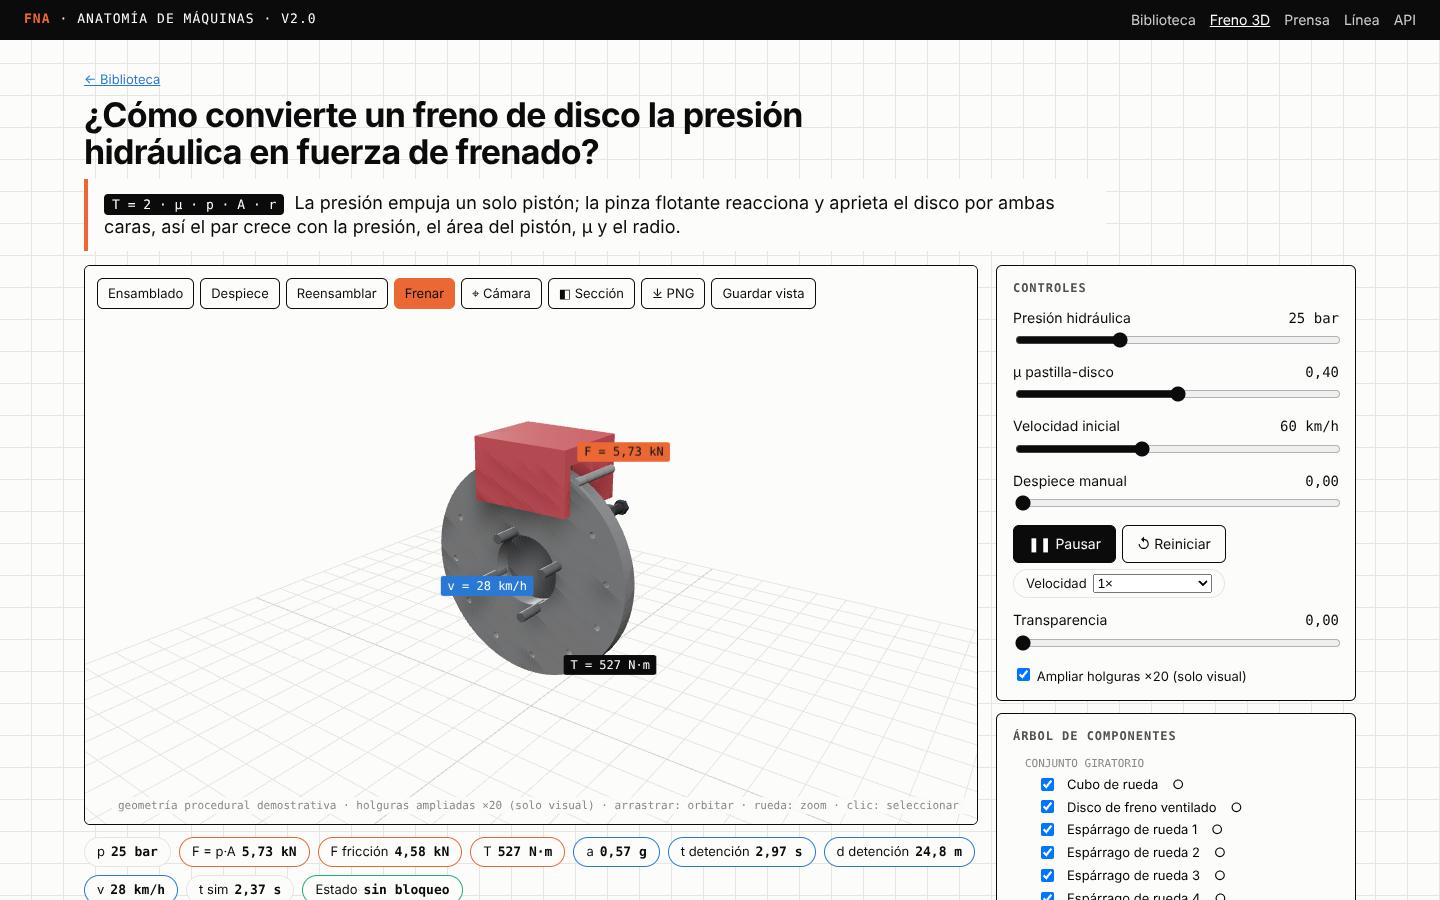
\includegraphics[width=\linewidth]{../capturas/v2/05_freno_frenado.png}}{\fbox{Captura no disponible}}
\caption{Freno en modo frenado: cifras junto a las piezas, lecturas y pasos del mecanismo}\label{fig:v2-frenado}
\end{figure}
\begin{figure}[H]\centering
\IfFileExists{../capturas/v2/03_freno_despiece.png}{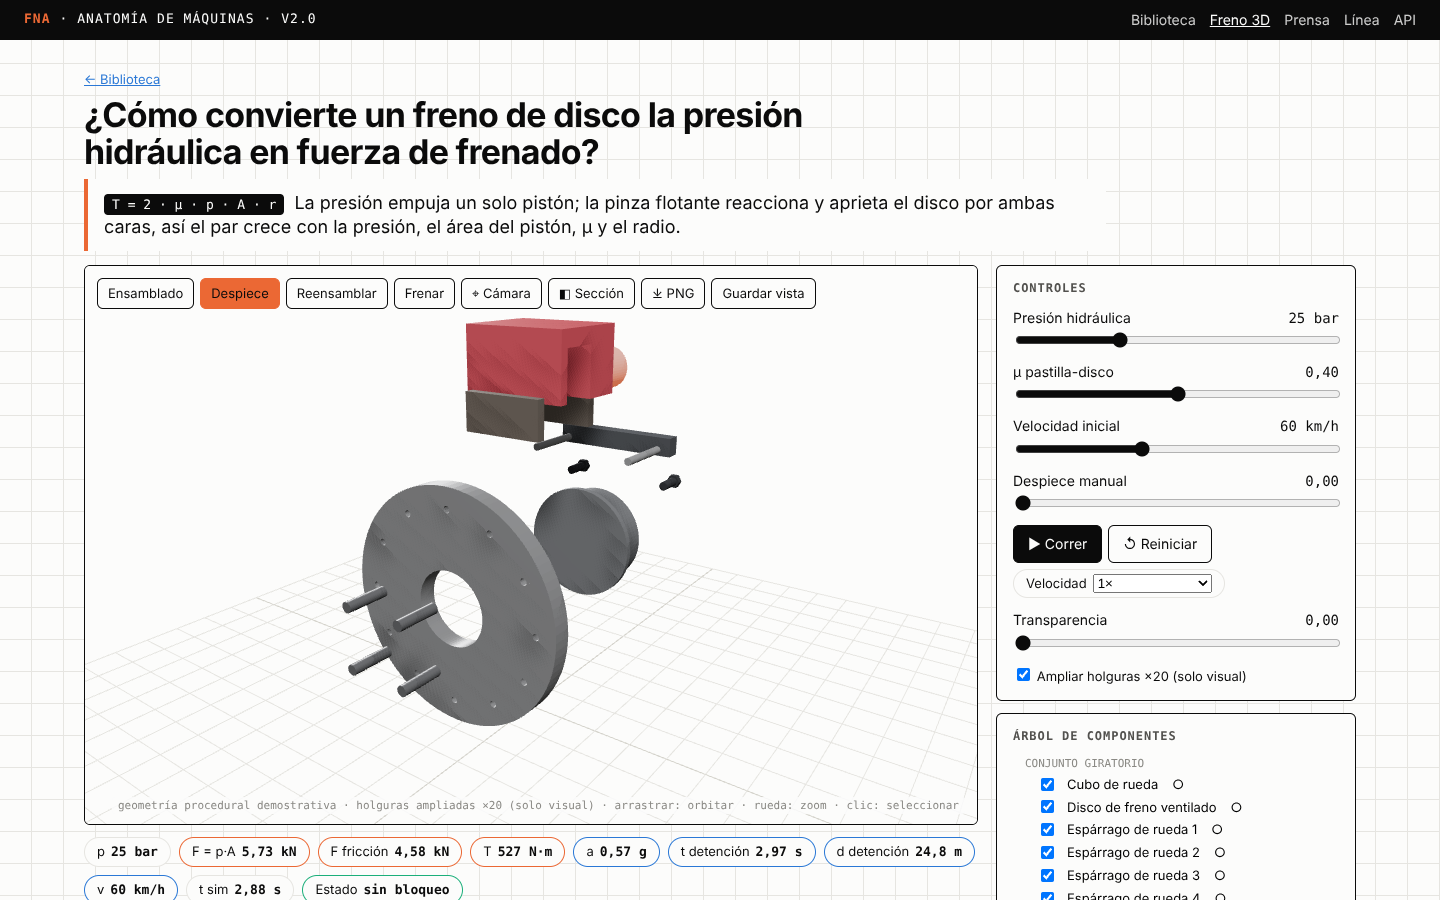
\includegraphics[width=0.49\linewidth]{../capturas/v2/03_freno_despiece.png}}{}\hfill
\IfFileExists{../capturas/v2/04_freno_seccion.png}{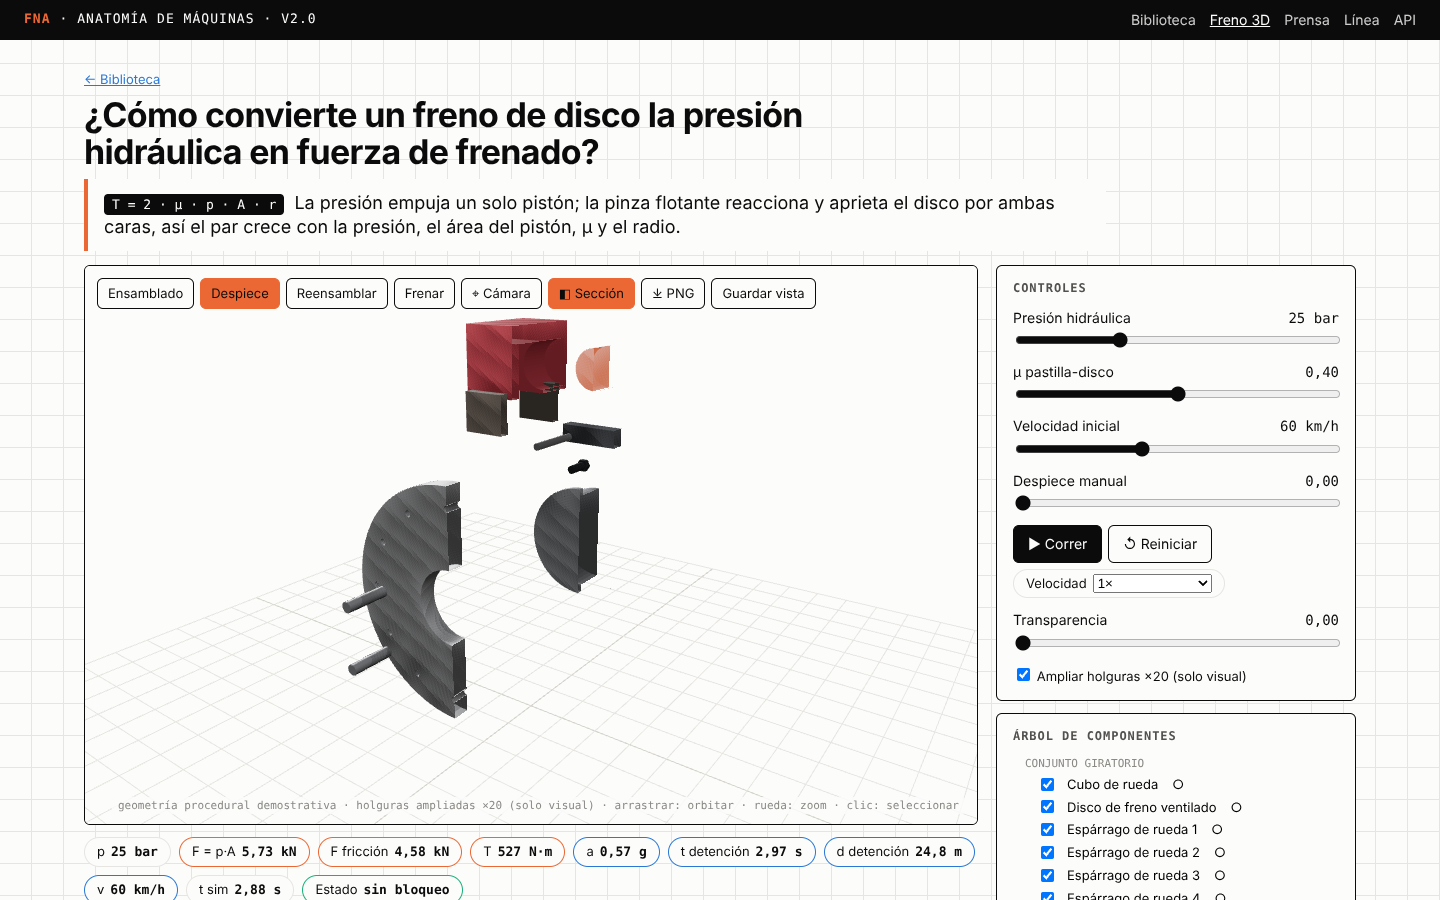
\includegraphics[width=0.49\linewidth]{../capturas/v2/04_freno_seccion.png}}{}
\caption{Vista de despiece (izquierda) y vista de sección (derecha)}\label{fig:v2-despiece}
\end{figure}

\begin{table}[H]\centering\small
\caption{Funciones del visor exigidas y su implementación}\label{tab:sim-visor}
\begin{tabularx}{\linewidth}{@{}P{3.6cm} X@{}}\toprule
Función & Implementación\\\midrule
Órbita, zoom, reinicio de cámara & \texttt{OrbitControls} (drei) con amortiguación; botón \emph{Cámara} ejecuta \texttt{reset()}.\\
Selección y árbol & Clic en la malla (raycasting) o en el árbol por subconjunto; resaltado emisivo.\\
Panel de información & Ficha: función, material demostrativo, dimensiones, retirar antes, relacionadas, procedencia.\\
Modos y velocidad & Ensamblado, despiece, reensamblaje, frenado y despiece manual; 1×, 0,5×, 0,25×, 0,1×.\\
Visibilidad y transparencia & Casilla por pieza, aislamiento, \emph{Mostrar todo}; opacidad 0--0,9.\\
Vista de sección & Plano de corte $x = 0$ con caras dobles.\\
Captura & Exportación PNG del lienzo (\texttt{preserveDrawingBuffer}).\\
Lecturas & Posición y ángulo de la pieza seleccionada (escena) y validación en la API.\\
Preguntas & Panel RAG con preguntas sugeridas y libres.\\
Estados & \emph{Guardar vista} en \texttt{/estados}; eventos de selección, despiece, visibilidad y captura.\\\bottomrule
\end{tabularx}
\end{table}

\section{Pruebas de la versión 2.0}
\begin{table}[H]\centering\small
\caption{Pruebas del simulador por categoría exigida}\label{tab:sim-pruebas}
\begin{tabularx}{\linewidth}{@{}P{3.4cm} X@{}}\toprule
Categoría & Pruebas\\\midrule
Jerarquía e identificadores & \texttt{test\_jerarquia\_cubre\_todas\_las\_piezas}, \texttt{test\_identificadores\_unicos\_y\_campos\_obligatorios}\\
Transformaciones & \texttt{test\_rotacion\_de\_rueda\_arrastra\_disco\_y\_esparragos}, \texttt{test\_euler\_ida\_y\_vuelta}, \texttt{test\_pinza\_flotante\_aprieta\_por\_ambas\_caras}\\
Límites & \texttt{test\_limites\_de\_articulacion}, \texttt{test\_cinematica\_valida\_limites}\\
Reversibilidad & \texttt{test\_despiece\_reversible\_y\_monotono}, \texttt{test\_secuencias\_desmontaje\_y\_reensamblaje}\\
Carga del modelo & \texttt{test\_glb\_carga\_con\_nodos\_por\_pieza}, \texttt{test\_manifiesto\_completo\_y\_mallas\_cerradas}, \texttt{test\_generacion\_reproducible}\\
API y persistencia & \texttt{test\_api\_simulador.py}, \texttt{test\_postgresql.py}\\
Frontend & Vitest (22 pruebas: réplica TS frente a Python, prensa, línea, biblioteca, enrutador); Playwright (biblioteca, freno 3D, prensa y línea)\\
Rendimiento & Playwright mide FPS durante el frenado (umbral conservador con render por software)\\\bottomrule
\end{tabularx}
\end{table}
